Different materials reflect different frequencies of light better than others, creating an imbalance in the light's spectral power distribution. Our eyes pick up certain frequencies in different intensities, and our brains combine these signals to create color vision. 

We should first develop a (sort of) rigorous model on the set of colors and what ``operations'' you can do with them. 

\begin{definition}[Color Space] 
  Let $V$ be a topological vector space over $\mathbb{R}$.\footnote{We can think of $V$ as a set representing some idea that generalizes the concept of color, supporting scalar multiplication, inverse, etc.} A \textbf{color space} is an abelian group $(C, m)$, where 
  \begin{enumerate}
    \item $C$ is a convex subset of $V$ containing $0$. 
    \item $m$ is a continuous \textbf{color mixing} operator 
    \begin{equation}
      m: C \times C \to C, m(c_1, c_2) \coloneqq \frac{1}{2} (c_1 + c_2) 
    \end{equation}  
    which represents the new color $m(c_1, c_2)$ you get from mixing colors $c_1$ and $c_2$ in equal volume. It is closed under the convex set by definition and can be interpreted as the midpoint between two colors. 
  \end{enumerate}
\end{definition} 

One might ask what the dimension of $V$ is, and my answer is: we don't know and don't care. This is because eventually, we will be working only with $C$ and will be treating it as a group anyways. So a better representation using convex hulls is more practical. 

\begin{figure}[H]
  \centering 
  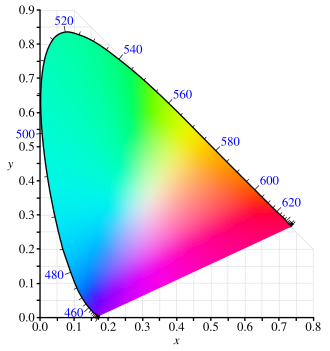
\includegraphics[scale=0.7]{img/horseshoe.png}
  \caption{The CIE 1931 color space depicts the color space of all visible colors to the human eye. The white background is the vector space $V$, and the ``horseshoe'' shaped set is $C$. It is the most popular visual of color spaces. Note that in this visual, we treat these colors as living in 2 dimensions.} 
  \label{fig:horseshoe}
\end{figure}

Note that this was quite an abstract definition, and we do this to construct a common interface between various color models. We have not stated what color each vector may represent (e.g. $0$ is what color?), nor have we defined what \textit{mixing} means (in terms of mixing paint or overlapping flashlight?). There are two broad categories that specify these. 

\begin{definition}[Additive Color Space] 
  In an \textbf{additive color space}, the 
  \begin{enumerate}
    \item $0$ vector is black. 
    \item $m(c_1, c_2)$ is the color you get when you shine two flashlights of colors $c_1$ and $c_2$---of equal intensity---into the same spot. 
  \end{enumerate}
  This is what you will probably use on a day-to-day basis. This is the standard for monitors specifications and visual design. 
\end{definition}

\begin{definition}[Subtractive Color Space]
  In a \textbf{subtractive color space}, the 
  \begin{enumerate}
    \item $0$ vector is white. 
    \item $m(c_1, c_2)$ is the color you get when you mix two paints of colors $c_1$ and $c_2$---of equal volume---into the same bucket. 
  \end{enumerate} 
  This is the norm for printers. 
\end{definition} 

Besides convexity, we don't really care about the vector space operations on $V$. We would like a more succinct representation of $C$. 

\begin{definition}[Gamut]
  The \textbf{gamut} of a finite set of colors $P = \{c_i \in V \}_{i=1}^n $ is the convex hull of $P$. A set of points $P$ is said to \textbf{generate} a color space $C$ if the convex hull of $P$ is $C$. 
\end{definition} 

\begin{definition}[Primary Colors]
  The \textbf{primary colors}, or \textbf{hues}, of a color space $C$ is any minimal\footnote{as in, we cannot generate the same space $C$ with a strict subset of $P$} set of points $P$ that generates $C$. 
\end{definition}

It is generally accepted that we need a set of 3 primary colors to accurately model the color space of visible colors. We mainly believe it to be 3 because the human eye has 3 main color receptors, but this has no strict justification. Which three primary colors we select determines the model. We will look at RGB, RYB, and CMY, which are the three most popular ones. 

\begin{definition}[Secondary Colors]
  Given a set of primary colors $P = \{p_1, p_2, p_3\}$ that generate a color space $(C, m)$, the \textbf{secondary colors} $S = \{s_1, s_2, s_3\}$ are defined 
  \begin{align}
    s_1 & = m(p_2, p_3) \\ 
    s_2 & = m(p_1, p_3) \\ 
    s_3 & = m(p_1, p_2) 
  \end{align}
\end{definition} 

\begin{figure}[H]
  \centering 
  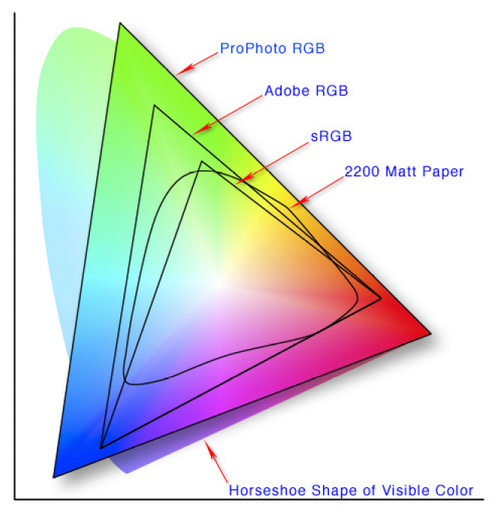
\includegraphics[scale=0.4]{img/colorspace.png}
  \caption{The gamut of visible colors w.r.t. the primary colors compared to gamuts of hardware in monitors. For visual convenience, all gamuts are projected into a 2-dimensional space.} 
  \label{fig:colorspace}
\end{figure} 

